%!TEX root = ../master.tex
\chapter{Code Overview}\label{ch:codeoverview}
\begin{figure}
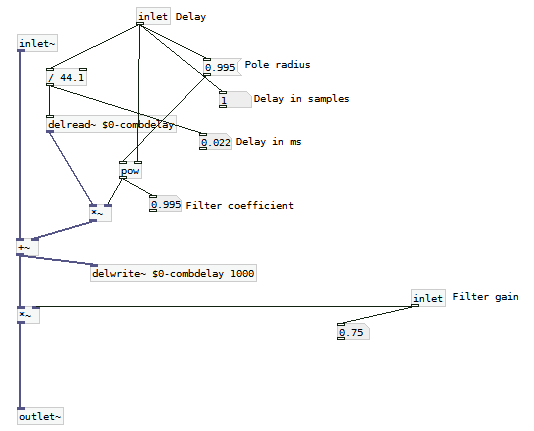
\includegraphics[width=0.5\textwidth]{Comb_filter}
\caption{Blocks inside the comb filter in pure data}
\label{Fig:Comb_filter}
\end{figure}

\begin{figure}
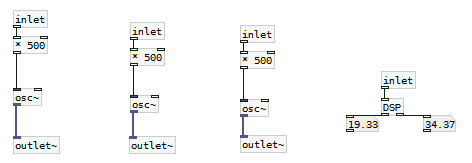
\includegraphics[width=0.5\textwidth]{Output}
\caption{The blocks that is inside the pd output block}
\label{Fig:Output}
\end{figure}



\section{Image processing code}
For the image processing a double nested for loop was implemented using an expr function in pure data. Making the for loop using three if statements instead of a for loop. The loop goes through 0 to 1, when it reaches 1 it adds 1 0.01 to another variable and resets to 0 to start over. When the second variable hits 1 it resets to 0 and the whole process starts over. This is visualised by the sliders in pure data, which moves in real time as the image is processed.  
The delay is placed so that the program doesn't preform a stack overflow when handling the if statements. 
\begin{figure}
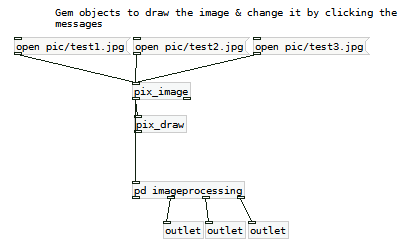
\includegraphics[width=0.5\textwidth]{Pdpictures}
\caption{The blocks that do imageprocessing}
\label{Fig:pdpicture}
\end{figure}

\begin{figure}
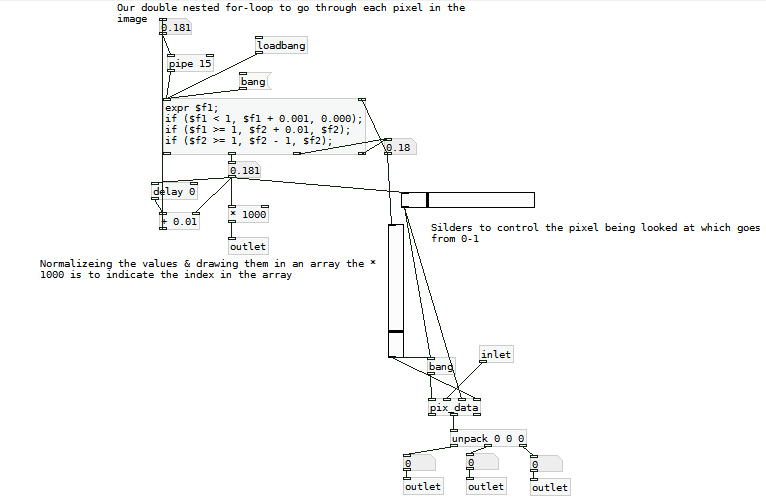
\includegraphics[width=0.5\textwidth]{Imageprocessing}
\caption{The blocks that is inside the pd imageprocessing block}
\label{Fig:Imageprocessing}
\end{figure}


\section{Filter code}


\section{Arduino code}

\begin{figure}
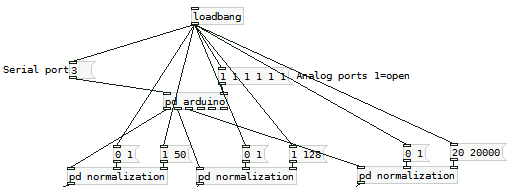
\includegraphics[width=0.5\textwidth]{Arduino_normalization}
\caption{The arduino blocks inputs and outputs}
\label{Fig:Arudino_normalization}
\end{figure}

\begin{figure}
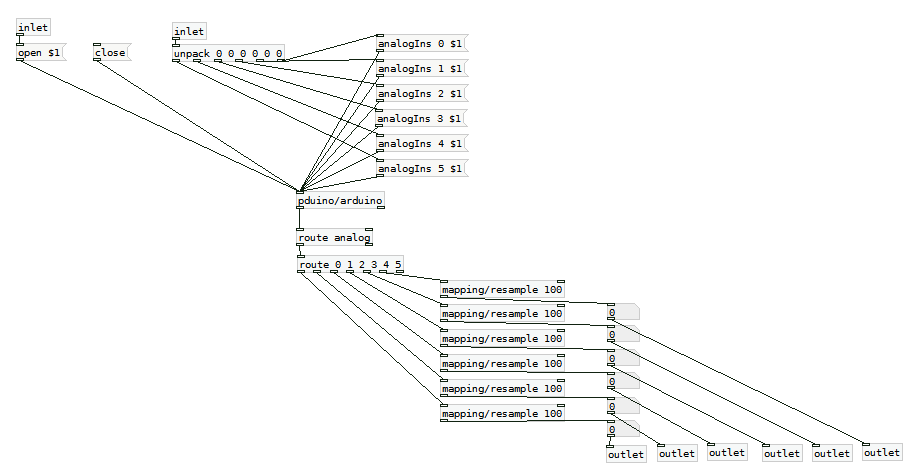
\includegraphics[width=0.5\textwidth]{Inside_arduino}
\caption{The blocks that is inside the pd arduino block}
\label{Fig:Inside_arduino}
\end{figure}

\begin{figure}
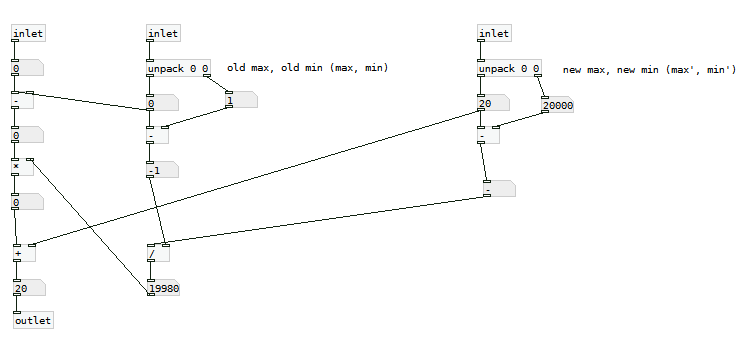
\includegraphics[width=0.5\textwidth]{Normalize}
\caption{The blocks inside the pd normalization block}
\label{Fig:Normalize}
\end{figure}